\chapter{Versuchsaufbau}
%
\begin{figure}[h]
    \centering
    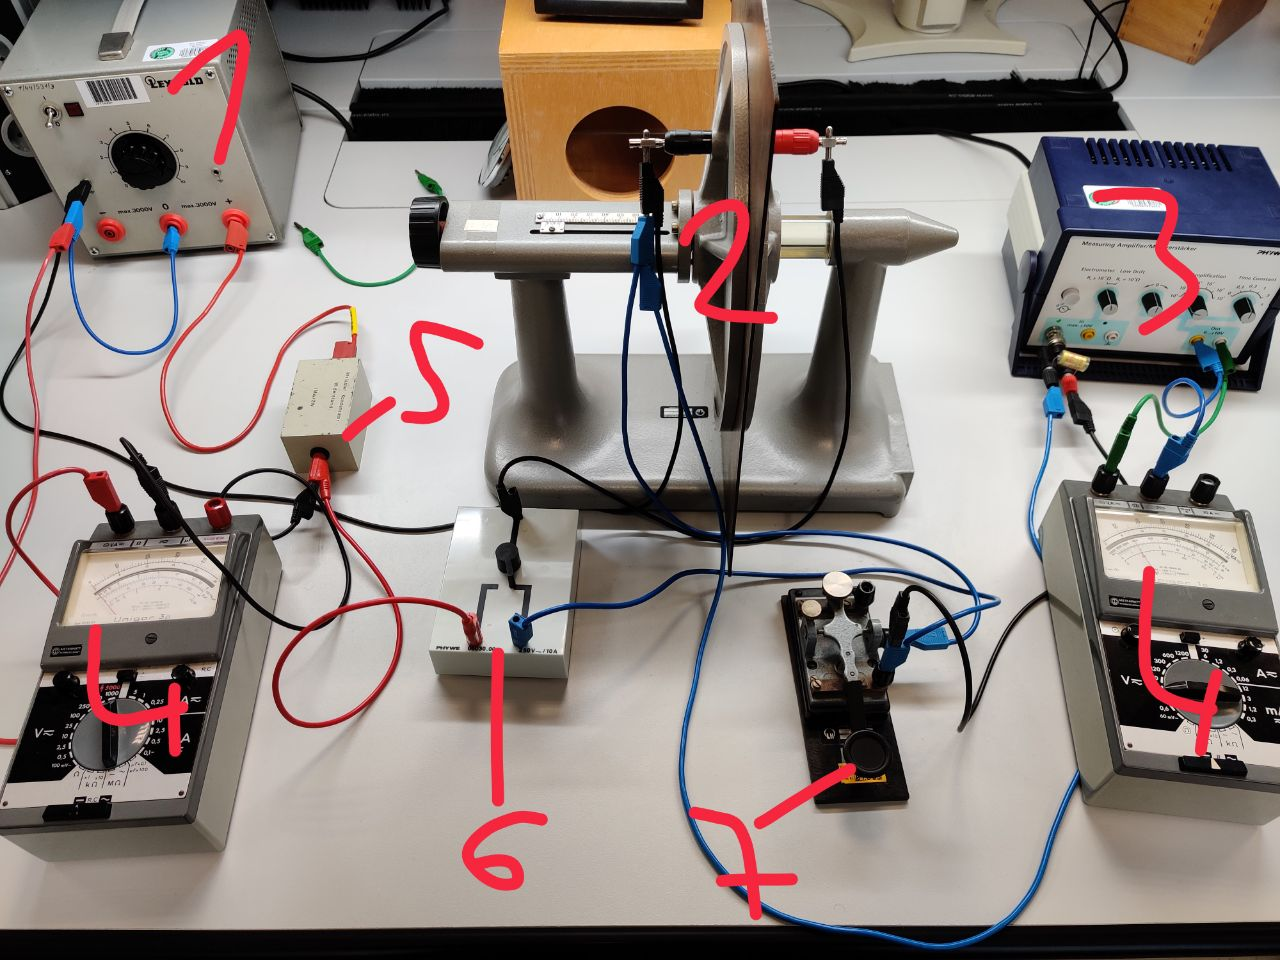
\includegraphics[width=\textwidth]{versuchsaufbau.jpg}
    \caption[Versuchsaufbau]{Versuchsaufbau mit variablem Kondensator und komplementären Geräten.
    1: Hochspannungsnetzteil,
    2: Variabler Kondensator $ C_{1} $ (links: geerdete Platte, rechts: isolierte Platte) mit Dielektrikum,
    3: Messverstärker des Herstellers \textit{PHYWE} mit Vergleichskondensator $ C_{2}=\SI{220}{nF}\cdot(1\pm10\%) $,
    4: Spannungsmessgerät (\textit{Unigor 3} zur Messung von $ U_{1} $, \textit{Unigor 1} zur Messung von $ U_{2} $),
    5: Vorwiderstand $ \SI{1}{M\ohm} $ im Gehäuse,
    6: Umschalter,
    7: Taster.
    }
    \label{fig:aufbau}
\end{figure}
%
\section{Messprinzip}
Das Hochspannungsnetzteil lädt den Kondensator $ C_{1} $ auf während das Messgerät die Spannung $ U_{1} $ misst.
Wird die Schaltung umgeschaltet, so entlädt der Vergleichskondensator $ C_{2} $ den ersten Kondensator $ C_{1} $. Die
dadurch verringerte Spannung wird vom zweiten Messgerät über den Messverstärker registriert. Wird der Umschalter wieder
betätigt, so lädt sich der Kondensator $ C_{1} $ wieder auf. Bedient man den Taster, dann entlädt sich der Kondensator
$ C_{2} $. Über das Verstellrad kann der Abstand $ d $ der Platten variiert und mit der Skala abgelesen werden.
\begin{figure}[h]
    \centering
    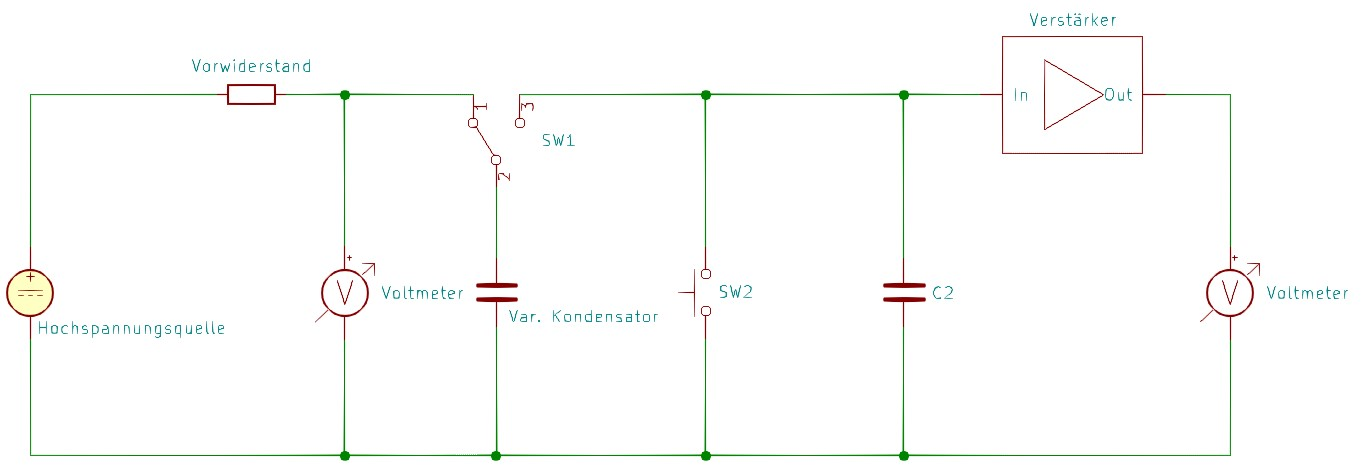
\includegraphics[width=\textwidth]{kicad/abbildungen/aufbau.jpg}
    \caption[Schaltskizze des Messaufbaus]{Schaltskizze des Messaufbaus.}
    \label{fig:schematic_aufbau}
\end{figure}